\documentclass{article}

\def \lastexercisenumber{20}

% Hier befinden sich Pakete, die wir beinahe immer benutzen ...

\usepackage[utf8]{inputenc}

% Sprach-Paket:
\usepackage[ngerman]{babel}

% damit's nicht so, wie beim Grill aussieht:
\usepackage{fullpage}

% Mathematik:
\usepackage{amsmath, amssymb, amsfonts, amsthm}
\usepackage{bbm}
\usepackage{mathtools, mathdots}

% Makros mit mehereren Default-Argumenten:
\usepackage{twoopt}

% Anführungszeichen (Makro \Quote{}):
\usepackage{babel}

% if's für Makros:
\usepackage{xifthen}
\usepackage{etoolbox}

% tikz ist kein Zeichenprogramm (doch!):
\usepackage{tikz}

% bessere Aufzählungen:
\usepackage{enumitem}

% (bessere) Umgebung für Bilder:
\usepackage{graphicx, subfig, float}

% Umgebung für Code:
\usepackage{listings}

% Farben:
\usepackage{xcolor}

% Umgebung für "plain text":
\usepackage{verbatim}

% Umgebung für mehrerer Spalten:
\usepackage{multicol}

% "nette" Brüche
\usepackage{nicefrac}

% Spaltentypen verschiedener Dicke
\usepackage{tabularx}
\usepackage{makecell}

% Für Vektoren
\usepackage{esvect}

% (Web-)Links
\usepackage{hyperref}

% Zitieren & Literatur-Verzeichnis
\usepackage[style = authoryear]{biblatex}
\usepackage{csquotes}

% so ähnlich wie mathbb
%\usepackage{mathds}

% Keine Ahnung, was das macht ...
\usepackage{booktabs}
\usepackage{ngerman}
\usepackage{placeins}

% special letters:

\newcommand{\N}{\mathbb{N}}
\newcommand{\Z}{\mathbb{Z}}
\newcommand{\Q}{\mathbb{Q}}
\newcommand{\R}{\mathbb{R}}
\newcommand{\C}{\mathbb{C}}
\newcommand{\K}{\mathbb{K}}
\newcommand{\T}{\mathbb{T}}
\newcommand{\E}{\mathbb{E}}
\newcommand{\V}{\mathbb{V}}
\renewcommand{\S}{\mathbb{S}}
\renewcommand{\P}{\mathbb{P}}
\newcommand{\1}{\mathbbm{1}}

% quantors:

\newcommand{\Forall}{\forall \,}
\newcommand{\Exists}{\exists \,}
\newcommand{\ExistsOnlyOne}{\exists! \,}
\newcommand{\nExists}{\nexists \,}
\newcommand{\ForAlmostAll}{\forall^\infty \,}

% MISC symbols:

\newcommand{\landau}{{\scriptstyle \mathcal{O}}}
\newcommand{\Landau}{\mathcal{O}}


\newcommand{\eps}{\mathrm{eps}}

% graphics in a box:

\newcommandtwoopt
{\includegraphicsboxed}[3][][]
{
  \begin{figure}[!h]
    \begin{boxedin}
      \ifthenelse{\isempty{#1}}
      {
        \begin{center}
          \includegraphics[width = 0.75 \textwidth]{#3}
          \label{fig:#2}
        \end{center}
      }{
        \begin{center}
          \includegraphics[width = 0.75 \textwidth]{#3}
          \caption{#1}
          \label{fig:#2}
        \end{center}
      }
    \end{boxedin}
  \end{figure}
}

% braces:

\newcommand{\pbraces}[1]{{\left  ( #1 \right  )}}
\newcommand{\bbraces}[1]{{\left  [ #1 \right  ]}}
\newcommand{\Bbraces}[1]{{\left \{ #1 \right \}}}
\newcommand{\vbraces}[1]{{\left  | #1 \right  |}}
\newcommand{\Vbraces}[1]{{\left \| #1 \right \|}}
\newcommand{\abraces}[1]{{\left \langle #1 \right \rangle}}
\newcommand{\round}[1]{\bbraces{#1}}

\newcommand
{\floorbraces}[1]
{{\left \lfloor #1 \right \rfloor}}

\newcommand
{\ceilbraces} [1]
{{\left \lceil  #1 \right \rceil }}

% special functions:

\newcommand{\norm}  [2][]{\Vbraces{#2}_{#1}}
\newcommand{\diam}  [2][]{\mathrm{diam}_{#1} \: #2}
\newcommand{\diag}  [1]{\mathrm{diag} \: #1}
\newcommand{\dist}  [1]{\mathrm{dist} \: #1}
\newcommand{\mean}  [1]{\mathrm{mean} \: #1}
\newcommand{\erf}   [1]{\mathrm{erf} \: #1}
\newcommand{\id}    [1]{\mathrm{id} \: #1}
\newcommand{\sgn}   [1]{\mathrm{sgn} \: #1}
\newcommand{\supp}  [1]{\mathrm{supp} \: #1}
\newcommand{\arsinh}[1]{\mathrm{arsinh} \: #1}
\newcommand{\arcosh}[1]{\mathrm{arcosh} \: #1}
\newcommand{\artanh}[1]{\mathrm{artanh} \: #1}
\newcommand{\card}  [1]{\mathrm{card} \: #1}
\newcommand{\Span}  [1]{\mathrm{span} \: #1}
\newcommand{\Aut}   [1]{\mathrm{Aut} \: #1}
\newcommand{\End}   [1]{\mathrm{End} \: #1}
\newcommand{\ggT}   [1]{\mathrm{ggT} \: #1}
\newcommand{\kgV}   [1]{\mathrm{kgV} \: #1}
\newcommand{\ord}   [1]{\mathrm{ord} \: #1}
\newcommand{\grad}  [1]{\mathrm{grad} \: #1}
\newcommand{\ran}   [1]{\mathrm{ran} \: #1}
\newcommand{\graph} [1]{\mathrm{graph} \: #1}
\newcommand{\Inv}   [1]{\mathrm{Inv} \: #1}
\newcommand{\pv}    [1]{\mathrm{pv} \: #1}
\newcommand{\GL}    [1]{\mathrm{GL} \: #1}
\newcommand{\Mod}{\mathrm{Mod} \:}
\newcommand{\Th}{\mathrm{Th} \:}
\newcommand{\Char}{\mathrm{char}}
\newcommand{\At}{\mathrm{At}}
\newcommand{\Ob}{\mathrm{Ob}}
\newcommand{\Hom}{\mathrm{Hom}}
\newcommand{\orthogonal}[3][]{#2 ~\bot_{#1}~ #3}
\newcommand{\Rang}{\mathrm{Rang}}
\newcommand{\NIL}{\mathrm{NIL}}
\newcommand{\Res}{\mathrm{Res}}
\newcommand{\lxor}{\dot \lor}
\newcommand{\Div}{\mathrm{div} \:}
\newcommand{\meas}{\mathrm{meas} \:}

% fractions:

\newcommand{\Frac}[2]{\frac{1}{#1} \pbraces{#2}}
\newcommand{\nfrac}[2]{\nicefrac{#1}{#2}}

% derivatives & integrals:

\newcommandtwoopt
{\Int}[4][][]
{\int_{#1}^{#2} #3 ~\mathrm{d} #4}

\newcommandtwoopt
{\derivative}[3][][]
{
  \frac
  {\mathrm{d}^{#1} #2}
  {\mathrm{d} #3^{#1}}
}

\newcommandtwoopt
{\pderivative}[3][][]
{
  \frac
  {\partial^{#1} #2}
  {\partial #3^{#1}}
}

\newcommand
{\primeprime}
{{\prime \prime}}

\newcommand
{\primeprimeprime}
{{\prime \prime \prime}}

% Text:

\newcommand{\Quote}[1]{\glqq #1\grqq{}}
\newcommand{\Text}[1]{{\text{#1}}}
\newcommand{\fastueberall}{\text{f.ü.}}
\newcommand{\fastsicher}{\text{f.s.}}

% -------------------------------- %
% amsthm-stuff:

\theoremstyle{definition}

% numbered theorems
\newtheorem{theorem}{Satz}
\newtheorem{lemma}{Lemma}
\newtheorem{corollary}{Korollar}
\newtheorem{proposition}{Proposition}
\newtheorem{remark}{Bemerkung}
\newtheorem{definition}{Definition}
\newtheorem{example}{Beispiel}

% unnumbered theorems
\newtheorem*{theorem*}{Satz}
\newtheorem*{lemma*}{Lemma}
\newtheorem*{corollary*}{Korollar}
\newtheorem*{proposition*}{Proposition}
\newtheorem*{remark*}{Bemerkung}
\newtheorem*{definition*}{Definition}
\newtheorem*{example*}{Beispiel}

% Please define this stuff in project ("main.tex"):

% \def \lastexercisenumber {...}
% This will be 0 by default

% \setcounter{section}{...}
% This will be 0 by default
% and hence, completely ignored

\ifnum \thesection = 0
{\newtheorem{exercise}{Aufgabe}}
\else
{\newtheorem{exercise}{Aufgabe}[section]}
\fi

\ifdef
{\lastexercisenumber}
{\setcounter{exercise}{\lastexercisenumber}}

\newcommand{\solution}
{
    \renewcommand{\proofname}{Lösung}
    \renewcommand{\qedsymbol}{}
    \proof
}

\renewcommand{\proofname}{Beweis}

% -------------------------------- %
% environment zum einkasteln:

% dickere vertical lines
\newcolumntype
{x}
[1]
{!{\centering\arraybackslash\vrule width #1}}

% environment selbst (the big cheese)
\newenvironment
{boxedin}
{
  \begin{tabular}
  {
    x{1 pt}
    p{\textwidth}
    x{1 pt}
  }
  \Xhline
  {2 \arrayrulewidth}
}
{
  \\
  \Xhline{2 \arrayrulewidth}
  \end{tabular}
}

% -------------------------------- %
% MISC "Ein-Deutschungen"

\renewcommand
{\figurename}
{Abbildung}

\renewcommand
{\tablename}
{Tabelle}

% -------------------------------- %


\addbibresource{../../../Fundament-LaTeX/references.bib}

\graphicspath{{../../../Fundament-LaTeX/images/}}

\parindent 0pt

\title
{
  Numerik von Partiellen Differentialgleichungen: stationäre Probleme \\
  \vspace{4pt}
  \normalsize
  \textit{5. Übung am 09.12.2020}
}
\author
{
  Richard Weiss
  \and
  Florian Schager
  \and
  Christian Sallinger
  %\and
  %Fabian Zehetgruber
  %\and
  %Paul Winkler
  %\and
  %Christian Göth
}
\date{}

\begin{document}

\maketitle

% --------------------------------------------------------------------------------

\begin{exercise}

Sei $A \in \R^{2 \times 2}$ eine symmetrische, positiv definite Matrix, $b \in \R^2$ und $c > 0$ mit $c - \frac{1}{2}\Div(b) \geq 0$.
Weiter seien $\Omega \subset \R^2$ ein beschränktes Lipschitz-Gebiet und $f \in L^2(\Omega)$.

\begin{enumerate}[label = \textbf{\alph*)}]

  \item Beweisen Sie, dass eine eindeutige schwache Lösung $u \in H_0^1(\Omega)$ von

  \begin{subequations}
    \begin{align}
      -\Div(A\nabla u) + b \cdot \nabla u + cu &= f \qquad \text{auf } \Omega, \label{eq:1A} \\
      u &= 0 \qquad \text{auf } \partial\Omega, \label{eq:1B}
    \end{align}
  \end{subequations}

  existiert.

  \item Sei $u_h \in \mathcal{S}_0^1(\mathcal{T})$ die eindeutige, schwache Finite-Elemente Lösung.
  Konstruieren Sie einen residualen Fehlerschätzer für
  $\norm[H_0^1(\Omega)]{u - u_h}$.

  \item Beweisen Sie, dass dieser Fehlerschätzer zuverlässig ist.

\end{enumerate}

\textit{Hinweis:}
Zeigen Sie zuerst, dass die zugehörige Bilinearform elliptisch ist.

\end{exercise}

% --------------------------------------------------------------------------------

\begin{solution}

Wir stellen zuerst das Funktional und die Bilinearform für die schwache Formlierung der PDE (1) auf.
$\Forall v \in H_0^1(\Omega):$

\begin{align*}
  F(v)
  & :=
  \Int[\Omega]{f v}{x}
  \stackrel{!}{=}
  \Int[\Omega]{(-\Div(A \nabla u) + b \cdot \nabla u + c u) v}{x}
  =
  -\Int[\Omega]{\Div(A \nabla u) v}{x}
  +
  \Int[\Omega]{(b \cdot \nabla u + c u) v}{x} \\
  & \stackrel
  {
    \mathrm{PI}
  }{=}
  \Int[\Omega]{A \nabla u \cdot \nabla v}
  -
  \underbrace
  {
    \Int[\partial \Omega]{(A \nabla u \cdot \nu) v}{s}
  }_0
  +
  \Int[\Omega]{(b \cdot \nabla u + c u) v}{x}
  =
  \Int[\Omega]{(\nabla u, \nabla v)_A + (b \cdot \nabla u + c u) v}{x} \\
  & =:
  a(u, v)
\end{align*}

Weil $\R^2$ endlich-dimensional ist, ist die, wegen der Symmetrie und positiven Definitheit von $A$ wohldefinierte, Energie-Norm $\norm[A]{\cdot}$ äquivalent zur Euklid-Norm $|\cdot|$.

\begin{align*}
  \implies
  \Exists \alpha, \beta > 0:
  \alpha |\cdot| \leq \norm[A]{\cdot} \leq \beta |\cdot|
\end{align*}

\begin{enumerate}[label = \textbf{\alph*)}]

  \item Wir wollen Exercise 7.2 (Lemma of Lax-Milgram) auf $F$ und $a$ anwenden.
  
  \begin{enumerate}[label = \arabic*.]

    \item $a$ stetig:
    
    \begin{align*}
      a(u, v)
      & =
      \Int[\Omega]{(\nabla u, \nabla v)_A + (b \cdot \nabla u + c u) v}{x}
      \stackrel
      {
        \mathrm{CSB}
      }{\leq}
      \Int[\Omega]{\norm[A]{\nabla u} \norm[A]{\nabla v} + |b| |\nabla u| v + c u v}{x} \\
      & \stackrel
      {
        \mathrm{CSB}
      }{\leq}
      \beta^2 \Int[\Omega]{|\nabla u| |\nabla v|}{x}
      +
      \norm[L^\infty]{b} \Int[\Omega]{|\nabla u| |v|}{x}
      +
      c \Int[\Omega]{u v}{x} \\
      & \leq
      \beta^2 \norm[L^2(\Omega)]{\nabla u} \norm[L^2(\Omega)]{\nabla v}
      +
      \norm[L^\infty(\Omega)]{b} \norm[L^2(\Omega)]{\nabla u} \norm[L^2(\Omega)]{v}
      +
      c \norm[L^2(\Omega)]{u} \norm[L^2(\Omega)]{v} \\
      & \leq
      \max \Bbraces{\beta^2, \norm[L^\infty(\Omega)]{b}, c} \norm[H^1(\Omega)]{u} \norm[H^1(\Omega)]{v}
    \end{align*}

    \item $a$ elliptisch:
    
    Die Produktregel für $\Div$ liefert uns
    
    \begin{align*}
      \Div(u^2 b) = \nabla(u^2) b + u^2 \Div b = 2 u b \nabla u + u^2 \Div b
      \implies
      u b \cdot \nabla u = \frac{1}{2} (\Div(u^2 b) - u \Div b),
    \end{align*}

    und der Integral-Satz von Gauß, dass ($u \in H_0^1(\Omega)$)

    \begin{align*}
      \Int[\Omega]{\Div (u^2 b)}{x}
      =
      \Int[\partial \Omega]{u^2 b \cdot \nu}{s}
      =
      0.
    \end{align*}

    Wir verwenden die Poincaré-Ungleichung.

    \includegraphicsboxed{PDEs/PDEs_-_Satz_5-11_(Poincare-Ungleichung).png}

    \begin{align*}
      \implies
      a(u, u)
      & =
      \Int[\Omega]{(\nabla u, \nabla u)_A + (b \cdot \nabla u + c u) v}{x}
      =
      \Int[\Omega]{\norm[A]{u}^2 + u b \cdot \nabla u + c u^2}{x} \\
      & \geq
      \Int[\Omega]{\alpha^2 |\nabla u|^2 + \frac{1}{2} (\Div(u^2 b) - u \Div b) + c u^2}{x} \\
      & =
      \alpha^2 \norm[L^2(\Omega)]{\nabla u}^2
      +
      \frac{1}{2} \Int[\partial \Omega]{u^2 b \cdot \nu}{s}
      +
      \underbrace
      {
        \Int[\Omega]{\pbraces{c - \frac{1}{2} \Div b} u^2}{x}
      }_{
        \geq 0
      } \\
      & \geq
      \alpha^2 \norm[L^2(\Omega)]{\nabla u}^2
      \geq
      \pbraces{\frac{\alpha}{C_P}}^2 \norm[H^1(\Omega)]{u}^2
    \end{align*}

  \end{enumerate}

  \item Siehe \textbf{c)} ...
  
  \item Wir formulieren ein Analogon zu Theorem 4.11.
  
  \includegraphicsboxed{NumPDEs/NumPDEs - Theorem 4.11.png}

  \begin{tcolorbox}[standard jigsaw, opacityback = 0]
    \textbf{Theorem 4.11. (Hier könnte Ihre Werbung stehen!)}
    Der Fehlerschätzer

    \begin{align*}
      \eta
      :=
      \pbraces
      {
        \norm[L^2(\Omega)]{h_\mathcal{T} (f - b \cdot \nabla u_h - c u_h)}^2
        +
        \norm[L^2(\mathcal{E}_\Omega)]{h_\mathcal{E}^{1/2} \dbbraces{\partial_n u_h}}^2
      }^{1/2}
    \end{align*}

    genügt der Zuverlässigkeits-Abschätzung

    \begin{align*}
      \norm[H^1(\Omega)]{u - u_h}
      \leq
      C \eta,
    \end{align*}

    wobei die Konstante $C > 0$ von der $\gamma$-Form-Regularität von $\mathcal{T}$ abhängt.

  \end{tcolorbox}

  \textbf{Beweis.}
  Für alle $w \in H_D^1(\Omega)$ und $T \in \mathcal{T}$, führt partielle Integration, und die Tatsache, dass $u_h \in \mathcal{S}^1(\Omega)$ und $A$ konstant ist, zu

  \begin{multline*}
    \Int[T]{(\nabla u_h, \nabla w)_A + (b \cdot \nabla u_h + c u_h) w}{x}
    =
    \Int[T]{A \nabla u_h \cdot \nabla w}{x}
    +
    \Int[T]{(b \cdot \nabla u_h + c u_h) w}{x} \\
    \stackrel
    {
      \mathrm{PI}
    }{=}
    -\Int[T]
    {
      \underbrace
      {
        \Div(A \nabla u_h)
      }_0
      w
    }{x}
    +
    \Int[\partial T]{\partial_n(A u_h) w}{s}
    +
    \Int[T]{(b \cdot \nabla u_h + c u_h) w}{x}.
  \end{multline*}

  Wir erinnern uns an die Definition vom \Quote{Sprung der Normalen-Ableitung}.

  \includegraphicsboxed{NumPDEs/NumPDEs - (4.34).png}

  \begin{align*}
    \implies
    R_h(w)
    & :=
    F(w) - a(u_h, w)
    =
    (f; w)_{L^2(\Omega)}
    -
    \sum_{T \in \mathcal{T}}
    \Int[T]{(\nabla u_h, \nabla w)_A + (b \cdot \nabla u_h + c u_h) w}{x} \\
    & =
    (f - b \cdot \nabla u_h - c u_h; w)_{L^2(\Omega)}
    -
    \sum_{T \in \mathcal{T}}
    (\partial_n (A u_h); w)_{L^2(\partial T)} \\
    & =
    \sum_{T \in \mathcal{T}}
    (f - b \cdot \nabla u_h - c u_h; w)_{L^2(T)} \\
    & -
    \underbrace
    {
      \sum_{E \in \mathcal{E}_D}
      (\partial_{n_E^-} (A u_h); w)_{L^2(E)}
    }_0
    -
    \sum_{E \in \mathcal{E}_\Omega}
    (\dbbraces{\partial_n (A u_h)}_E; w)_{L^2(E)} \\
    & \stackrel
    {
      \mathrm{CSB}
    }{\leq}
    \sum_{T \in \mathcal{T}}
    \norm[L^2(T)]{f - b \cdot \nabla u_h - c u_h}
    \norm[L^2(T)]{w}
    +
    \sum_{E \in \mathcal{E}_\Omega}
    \norm[L^2(E)]{\dbbraces{\partial_n u_h}_E}
    \norm[L^2(E)]{w}
  \end{align*}

  Für beliebiges $v \in H_D^1(\Omega)$, wählen wir nun $w = v - H_h v$ und bemerken, dass $R_h(v) = R_h(w)$, laut Galerkin Orthogonalität.

  \begin{align*}
    R_h(w)
    =
    R_h(v - J_h v)
    =
    R_h(v) - R_h(J_h v)
    =
    R_h(v) - \underbrace{a(u - u_h, J_h v)}_0
  \end{align*}

  Dann, schätzen wir die zwei Summen separat ab.

  \begin{tcolorbox}[standard jigsaw, opacityback = 0]
    \centering
    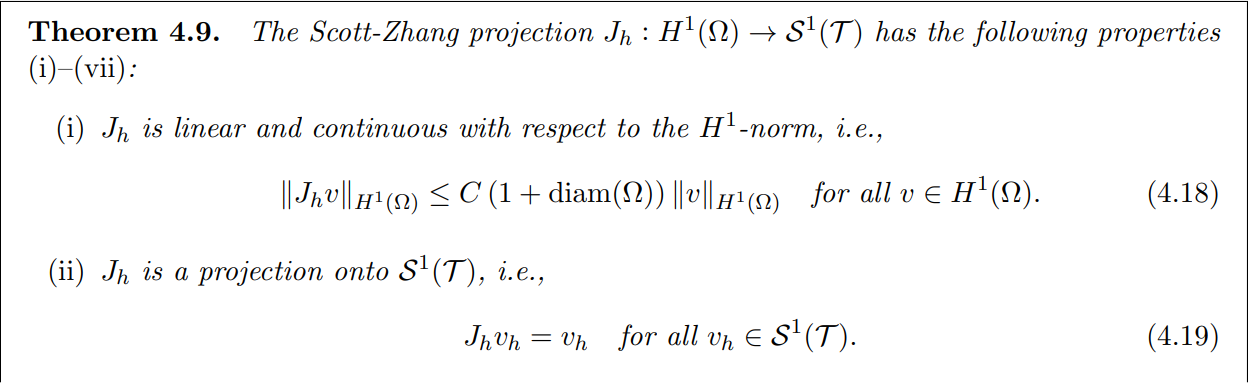
\includegraphics[width = 0.75 \textwidth]{NumPDEs/NumPDEs - Theorem 4.9.1.png} \\
    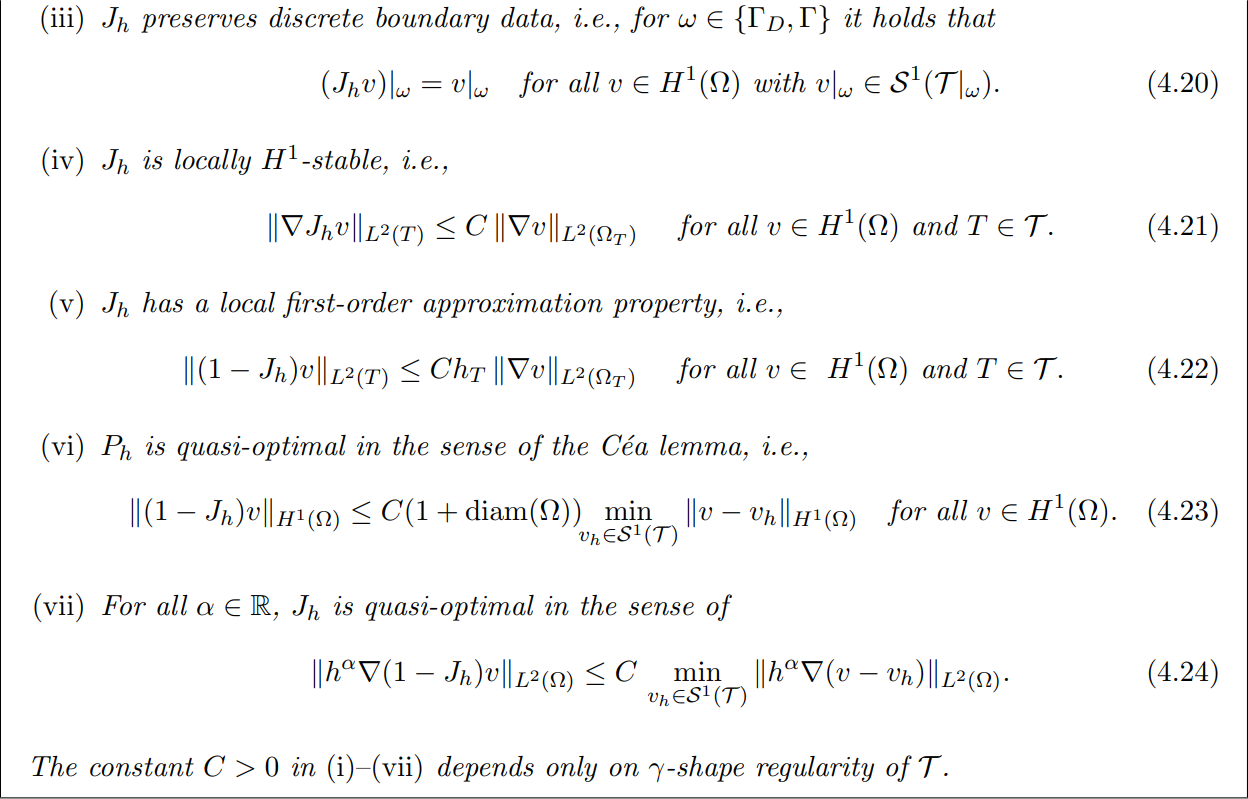
\includegraphics[width = 0.75 \textwidth]{NumPDEs/NumPDEs - Theorem 4.9.2.png}
  \end{tcolorbox}

  \begin{tcolorbox}[standard jigsaw, opacityback = 0]
    \centering
    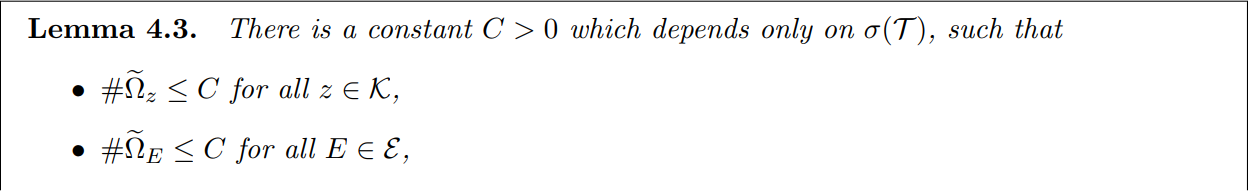
\includegraphics[width = 0.75 \textwidth]{NumPDEs/NumPDEs - Lemma 4.3.1.png} \\
    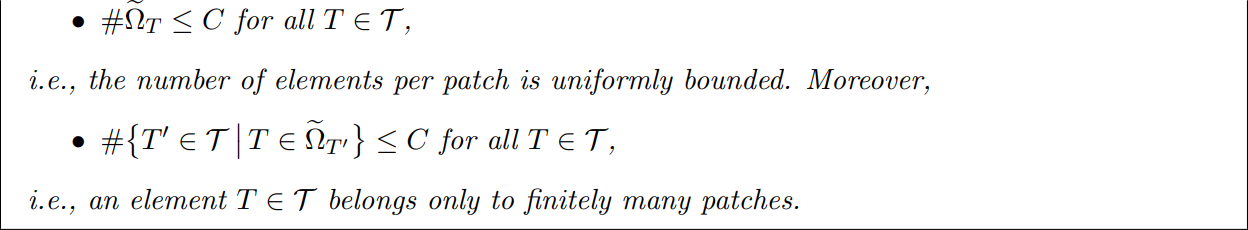
\includegraphics[width = 0.75 \textwidth]{NumPDEs/NumPDEs - Lemma 4.3.2.png}
  \end{tcolorbox}

  Die Approximations-Eigenschaft des Clément-Operators $J_h$, d.h. Lemma 4.9 (v) und der letzte Unterpunkt von Lemma 4.3 implizieren

  \begin{align*}
    & \sum_{T \in \mathcal{T}}
    \norm[L^2(T)]{f - (b \cdot \nabla u_h + c u_h)}
    \norm[L^2(T)]{v - J_h v} \\
    & \stackrel
    {
      \mathrm{4.9 (v)}
    }{\leq}
    \sum_{T \in \mathcal{T}}
    \norm[L^2(T)]{f - (b \cdot \nabla u_h + c u_h)}
    C_1 h_T
    \norm[L^2(\Omega_T)]{\nabla v} \\
    & \stackrel
    {
      \mathrm{CSB}
    }{\leq}
    C_1
    \pbraces
    {
      \sum_{T \in \mathcal{T}}
      \norm[L^2(T)]{h_\mathcal{T} (f - b \cdot \nabla u_h - c u_h)}^2
    }^{1/2}
    \pbraces
    {
      \sum_{T \in \mathcal{T}}
      \norm[L^2(\Omega_T)]{\nabla v}^2
    }^{1/2} \\
    & \stackrel
    {
      \mathrm{4.3}
    }{\leq}
    C_1 C_2
    \pbraces
    {
      \sum_{T \in \mathcal{T}}
      \norm[L^2(T)]{h_\mathcal{T} (f - b \cdot \nabla u_h - c u_h)}^2
    }^{1/2}
    \pbraces
    {
      \sum_{T \in \mathcal{T}}
      \norm[L^2(T)]{\nabla v}^2
    }^{1/2} \\
    & =
    C_1 C_2
    \norm[L^2(\Omega)]{h_\mathcal{T} (f - b \cdot \nabla u_h - c u_h)}
    \norm[L^2(\Omega)]{\nabla v}
  \end{align*}

  Für jede Kante $E \in \mathcal{E}$, wählen wir ein arbiträres Element $T_E \in \mathcal{T}$ mit $E \in \mathcal{E}_{T_E}$.
  Sei $\mathcal{E}_\ast \subset \mathcal{E}$ und $\psi \in L^2(E)$ für alle $E \in \mathcal{E}_\ast$.
  Man erinnere sich an Lemma 4.10.

  \includegraphicsboxed{NumPDEs/NumPDEs - Lemma 4.10.png}

  Daher, zeigen die selben Argumente wie zuvor, dass

  \begin{align*}
    \sum_{E \in \mathcal{E}_\ast}
    \norm[L^2(E)]{\psi}
    \norm[L^2(E)]{v - J_h v}
    & \stackrel
    {
      \mathrm{4.10}
    }{\leq}
    \sum_{E \in \mathcal{E}_\ast}
    \norm[L^2(E)]{\psi}
    C_3 h_E^{1/2}
    \norm[L^2(\Omega_{T_E})]{\nabla v} \\
    & \stackrel
    {
      \mathrm{CSB}
    }{\leq}
    C_3
    \pbraces
    {
      \sum_{E \in \mathcal{E}_\ast}
      \norm[L^2(E)]{h_\mathcal{E}^{1/2} \psi}^2
    }^{1/2}
    \pbraces
    {
      \sum_{E \in \mathcal{E}_\ast}
      \norm[L^2(\Omega_{T_E})]{\nabla v}^2
    }^{1/2} \\
    & \stackrel{!}{\leq}
    C_3
    \pbraces
    {
      \sum_{E \in \mathcal{E}_\ast}
      \norm[L^2(E)]{h_\mathcal{E}^{1/2} \psi}^2
    }^{1/2}
    \pbraces
    {
      3
      \sum_{T \in \mathcal{T}}
      \norm[L^2(T)]{\nabla v}^2
    }^{1/2} \\
    & =
    \sqrt{3} C_3
    \norm[L^2(\mathcal{E}_\ast)]{h_\mathcal{E}^{1/2} \psi}
    \norm[L^2(\Omega)]{\nabla v},
  \end{align*}

  wobei wir bemerken, dass ein Element $T \in \mathcal{T}$ nur $= T_E$ sein kann auf höchstens $3$ Kanten.
  Die Euklid-Norm ist zur Manhattan-Norm auf dem $\R^2$ äquivalent, vermöge $1$ bzw. $\sqrt{2}$.
  Insgesamt sehen wir nun ($\psi := \dbbraces{\partial_n u_h}$ und $\mathcal{E}_\ast := \mathcal{E}_\Omega)$)

  \begin{align*}
    R_h(v)
    & \leq
    C_1 C_2
    \norm[L^2(\Omega)]{h_\mathcal{T} (f - b \cdot \nabla u_h - c u_h)}
    \norm[L^2(\Omega)]{\nabla v}
    +
    \sqrt{3} C_3
    \norm[L^2(\mathcal{E}_\Omega)]{h_\mathcal{E}^{1/2} \dbbraces{\partial_n u_h}}
    \norm[L^2(\Omega)]{\nabla v} \\
    & \leq
    \max \Bbraces{C_1 C_2, \sqrt{3} C_3}
    \norm[L^2(\Omega)]{\nabla v}
    \pbraces
    {
      \norm[L^2(\Omega)]{h_\mathcal{T} (f - b \cdot \nabla u_h - c u_h)}
      +
      \norm[L^2(\mathcal{E}_\Omega)]{h_\mathcal{E}^{1/2} \dbbraces{\partial_n u_h}}
    } \\
    & \leq
    \max \Bbraces{C_1 C_2, \sqrt{3} C_3}
    \norm[L^2(\Omega)]{\nabla v}
    \sqrt{2}
    \pbraces
    {
      \norm[L^2(\Omega)]{h_\mathcal{T} (f - b \cdot \nabla u_h - c u_h)}^2
      +
      \norm[L^2(\mathcal{E}_\Omega)]{h_\mathcal{E}^{1/2} \dbbraces{\partial_n u_h}}^2
    }^{1/2} \\
    & \leq
    \sqrt{2}
    \max \Bbraces{C_1 C_2, \sqrt{3} C_3}
    \norm[L^2(\Omega)]{\nabla v}
    \eta.
  \end{align*}

  Nun gilt es, die Vorbemerkungen des Beweises von dem originalem Theorem 4.11 nachzubauen.
  Weil $v \in \in H_D^1(\Omega)$ beliebig war, folgt

  \begin{align*}
    \implies
    \sup_{w \in H_D^1(\Omega)}
    \frac
    {
      R_h(w)
    }{
      \norm[L^2(\Omega)]{\nabla w}
    }
    \leq
    \sqrt{2}
    \max \Bbraces{C_1 C_2, \sqrt{3} C_3}
    \eta.
  \end{align*}

  Nachdem $u \in H_D^1(\Omega)$ ja eine schwache Lösung ist,

  \begin{align*}
    \implies
    R_h(v)
    =
    F(v) - a(u_h, v)
    =
    \underbrace
    {
      F(v) - a(u, v)
    }_0
    +
    a(u, v)
    -
    a(u_h, v)
    =
    a(u - u_h, v).
  \end{align*}

  Es seien $L$ die Stetigkeits- und $M$ die Elliptizitäts-Konstante von $a$.

  \begin{multline*}
    M \norm[H^1(\Omega)]{u - u_h}
    =
    \frac
    {
      M \norm[H^1(\Omega)]{u - u_h}^2
    }{
      \norm[H^1(\Omega)]{u - u_h}
    }
    \leq
    \frac
    {
      M \norm[H^1(\Omega)]{u - u_h}^2
    }{
      \norm[L^2(\Omega)]{\nabla (u - u_h)}
    }
    \leq
    \frac
    {
      a(u - u_h, u - u_h)
    }{
      \norm[L^2(\Omega)]{\nabla (u - u_h)}
    } \\
    =
    \frac
    {
      R_h(u - u_h)
    }{
      \norm[L^2(\Omega)]{\nabla (u - u_h)}
    }
    \leq
    \sup_{w \in H_D^1(\Omega)}
    \frac
    {
      R_h(w)
    }{
      \norm[L^2(\Omega)]{\nabla w}
    }
  \end{multline*}

  Damit erhalten wir nun endlich unsere finale Abschätzung.

  \begin{align*}
    C
    :=
    \frac
    {
      \sqrt{2}
      \max \Bbraces{C_1 C_2, \sqrt{3} C_3}
    }{
      M
    }
    \implies
    \norm[H^1(\Omega)]{u - u_h}
    \leq
    C \eta
  \end{align*}

  Die (nicht versteckte) Konstante $C$ hängt nur ab (von dem Clemént-Operator $J_h$ und) von der $\gamma$-Form-Regularität von $\mathcal{T}$.

\end{enumerate}

\end{solution}

% --------------------------------------------------------------------------------

% -------------------------------------------------------------------------------- %

\begin{exercise}

Beweisen Sie die Aussage aus Ex. 26 des Vorlesungsskriptes.

\end{exercise}

% -------------------------------------------------------------------------------- %

\begin{solution}

\phantom{}

\end{solution}

% -------------------------------------------------------------------------------- %

% -------------------------------------------------------------------------------- %

\begin{exercise}

Beweisen Sie die Aussagen aus Ex. 29 und Ex. 30 des Vorlesungsskriptes.
\includegraphicsunboxed{NumPDEs/NumPDEs - Exercise 29}
\includegraphicsunboxed{NumPDEs/NumPDEs - Exercise 30}

\end{exercise}

% -------------------------------------------------------------------------------- %

\begin{solution}

\textit{Aufgabe 29.}

Dem Hinweis nach definieren wir

\begin{align*}
  \mathcal{X}_\infty
  :=
  \overline{\bigcup_{\ell=0}^\infty \mathcal{X}_\ell}
  \subset H
\end{align*}

Um die Aussage zu zeigen werden wir nun Proposition $1.7$ benutzen.

\includegraphicsunboxed{NumPDEs/NumPDEs - Proposition 1.7}

Da $\bigcup_{\ell \in \N} \mathcal{X}_\ell$ nach Konstruktion dicht in $\mathcal{X}_\infty$ liegen gilt es also zu zeigen:

\begin{align*}
  \forall v \in \bigcup_{\ell \in \N} \mathcal{X}_\ell: ~
  \lim_{\ell \to \infty} \min_{v_\ell \in \mathcal{X}_\ell}
  \norm[H]{v - v_\ell} = 0
\end{align*}

Sei also $v \in \bigcup_{\ell \in \N} \mathcal{X}_\ell$, dann gilt sicher

\begin{align*}
  \exists k \in \N: v \in \mathcal{X}_k,
\end{align*}

Weil diese Unterräume bezüglich $\subset$ aufsteigend angeordnet sind sogar

\begin{align*}
  \forall \ell \geq k: v \in \mathcal{X}_\ell
\end{align*}

Damit schließen wir, da das Minimum auf einem kleineren Raum stets größer ist

\begin{align*}
  \forall \ell \geq k: \quad
  \min_{v_\ell \in \mathcal{X}_\ell} \norm[H]{v - v_\ell}
  \leq
  \min_{v_k \in \mathcal{X}_k} \norm[H]{v - v_k}
  \leq
  \norm[H]{v-v}
  =
  0
\end{align*}

Da $\mathcal{X}_\infty \supseteq \mathcal{X}_l$ gilt
\begin{align*}
  \forall v \in \mathcal{X}_l: \langle \langle U_\infty; v \rangle \rangle =
  \langle \langle u; v \rangle \rangle
  = \langle \langle \mathbb{G}_l u; v \rangle \rangle
\end{align*}
und es folgt $\mathbb{G}_l(u) = \mathbb{G}_l(U_\infty)$ und es gilt nach Proposition $1.7$:

\begin{align*}
  \lim_{\ell \to \infty} ||U_\infty - \underbrace{\mathbb{G}_\ell U_\infty}_{U_\ell}||_H
  =
  0
\end{align*}

\textit{Aufgabe 30.}

Definieren wir $\mathcal{X}_\infty$ so wie im vorherigen Aufgabenteil. Dann gilt es zu zeigen

\begin{align*}
  \forall u \in H^1_D(\Omega):
  \exists (u_k)_{k \in \N} \in \Big(\bigcup_{\ell \in \N} \mathcal{S}^1_D(\mathcal{T}_\ell)\Big)^\N:
  \quad
  \lim_{k \to \infty} \norm[H^1(\Omega)]{u - u_k} = 0
\end{align*}

Da wir gleichmäßig verfeinern gilt, wenn wir mit $h_0 := \max_{T \in \mathcal{T}_0} \diam T$ bezeichnen

\begin{align*}
  \forall \ell \in \N:~
  h_\ell
  =
  \frac{h_0}{2^\ell}
\end{align*}

Es gilt ebenfalls

\begin{align*}
  \forall \ell \in \N:~
  \sigma(\mathcal{T}_\ell) = \sigma(\mathcal{T}_0)
\end{align*}

Für beliebiges $u \in H^1_D(\Omega) = \overline{C^\infty_D(\overline{\Omega})}^{||\cdot||_{H^1(\Omega)}}$ wollen wir nun wieder Proposition $1.7$ verwenden. Unseren dichten Teilraum für den wir die Approximationseigenschaft zeigen wollen haben wir nun schon bestimmt. Zusätzlich benötigen wir noch Korollar $3.6$ (wobei hier $C^\infty_D(\overline{\Omega}) \subset H^2(\Omega) \cap H^1_D(\Omega)$ mit eingeht).

\includegraphicsunboxed{NumPDEs/NumPDEs - Corollary 3.6}

Sei nun also $v \in C^\infty_D(\overline{\Omega})$, dann erhalten wir

\begin{align*}
  \min_{v_\ell \in \mathcal{S}^1_D(\mathcal{T}_\ell)} \norm[H^1(\Omega)]{v - v_\ell}
  \stackrel{3.6}{\leq}
  C \sigma(\mathcal{T}_\ell)\norm[L^2(\Omega)]{h_\ell D^2v}
  =
  C \sigma(\mathcal{T}_0) \frac{h_0}{2^\ell} \norm[L^2(\Omega)]{D^2v}
  \stackrel{\ell \to \infty}{\longrightarrow}
  0
\end{align*}

Damit gilt nach Proposition $1.7$ nun auch

\begin{align*}
  \lim_{k \to \infty} \|u - \underbrace{\mathbb{G}_ku}_{=:u_k}\|_{H^1(\Omega)} = 0
\end{align*}
\end{solution}

% -------------------------------------------------------------------------------- %

% --------------------------------------------------------------------------------

\begin{exercise}

Sei $u \in H_0^1(\Omega)$ für ein beschränktes Lipschitz-Gebiet $\Omega \subset \R^2$
die Lösung des Poisson-Problems
\begin{align}
  \forall v \in H_0^1(\Omega): (\nabla u;\nabla v)_{L^2(\Omega)} = (f;v)_{L^2(\Omega)}
\end{align}
und $u_h \in \mathcal{S}_0^1(\mathcal{T})$ die zugehörige diskrete Finite-Elemente Lösung.
Weiter sei $\mathcal{K}$ die Knotenmenge der Triangulierung $\mathcal{T}$,
$\zeta_z \in \mathcal{S}_0^1(\mathcal{T})$ für alle $z \in \mathcal{K}$ die Hutfunktionen,
$\tilde{\Omega}_z := \{T \in \mathcal{T}: z \in T\}$ der Knotenpatch aus Abschnitt 4.2 und
\begin{align}
  \tilde{v}_h := \sum_{z \in \mathcal{K}}\left(\frac{1}{|\tilde{\Omega}_z|}
  \sum_{T \in \tilde{\Omega}_z}\nabla u_h|_T\right)\zeta_z
\end{align}
der gemittelte Gradient von $u_h$.
\begin{enumerate}[label = \textbf{\alph*)}]
  \item Beweisen Sie, dass
  \begin{align}
    \eta_{ZZ} := \|\nabla u_h - \tilde{v}_h\|_{L^2(\Omega)}
  \end{align}
  ein zuverlässiger und effizienter Fehlerschätzer ist, wenn der gemittelte
  Gradient eine bessere Approximation an den echten Gradienten ist, als der
  Gradient der FE-Lösung, das heißt, wenn eine Konstante $\alpha < 1$ existiert,
  sodass
  \begin{align}
    \|\nabla u - \tilde{v}_h\|_{L^2(\Omega)} \leq \alpha\|\nabla u - \nabla u_h\|_{L^2(\Omega)}.
    \label{ineq_grad}
  \end{align}
  \item Implementieren Sie diesen Fehlerschätzer in NGSolve und testen Sie numerisch
  sowohl die Güte des Fehlerschätzers als auch die Ungleichung \eqref{ineq_grad}.
  Konstruieren Sie sich dazu analog zu Beispiel 10 geeignete Referenzlösungen. \\

  \textit{Hinweis:} In NGSolve ist $\tilde{v}_h$ sehr elegant mit den Code-Zeilen
  \begin{itemize}
    \item $\mathrm{fe\_ag = VectorH1(mesh, order = 1)}$
    \item $\mathrm{vtilde = GridFunction(fe\_ag)}$
    \item $\mathrm{flux = grad(gfu)}$
    \item $\mathrm{vtilde.Set(flux)}$
  \end{itemize}
  zu berechnen.
\end{enumerate}
\end{exercise}

% --------------------------------------------------------------------------------

\begin{solution}

\begin{enumerate}[label = \textbf{\alph*)}]
  \item Erinnern wir uns daran, was es heißt zuverlässig und effizient zu sein. Es gilt zu zeigen

  \begin{align*}
    \norm[H^1(\Omega)]{u - u_h} &\leq C_{\text{rel}}~ \eta_{ZZ} \\
    C_{\text{eff}}~ \eta_{ZZ} &\leq \norm[H^1(\Omega)]{u - u_h}
  \end{align*}

  Um die Effizienz zu zeigen können wir \ref{ineq_grad} direkt verwenden:

  \begin{align*}
    \eta_{ZZ}
    &=
    \norm[L^2(\Omega)]{\nabla u_h - \tilde{v}_h}
    \leq
    \norm[L^2(\Omega)]{\nabla u - \nabla u_h} + \norm[L^2(\Omega)]{\nabla u - \tilde{v}_h}
    \stackrel{\ref{ineq_grad}}{\leq}
    (1 + \alpha) \norm[L^2(\Omega)]{\nabla u - \nabla u_h} \\
    &\leq
    (1 + \alpha) \norm[H^1(\Omega)]{u - u_h}
  \end{align*}

  Für die Zuverlässigkeit multiplizieren wir \ref{ineq_grad} mit $-1$ und sehen dadurch

  \begin{align*}
    \norm[L^2(\Omega)]{\nabla u - \nabla u_h} - \norm[L^2(\Omega)]{\nabla u - \tilde{v}_h}
    \geq
    (1 - \alpha) \norm[L^2(\Omega)]{\nabla u - \nabla u_h}
  \end{align*}

  Damit, sowie mit der Poincare-Ungleichung schätzen wir nun ab:
  \includegraphicsboxed{PDEs/PDEs_-_Satz_5-11_(Poincare-Ungleichung)}
  \begin{align*}
    \norm[H^1{\Omega}]{u - u_h}
    &=
    \sqrt{\norm[L^2(\Omega)]{u - u_h}^2 + \norm[L^2(\Omega)]{\nabla u - \nabla u_h}^2}
    \leq
    \underbrace{\sqrt{(1+C_p^2)}}_{:=C} \norm[L^2(\Omega)]{\nabla u - \nabla u_h} \\
    &\leq
    \frac{C}{1-\alpha} \Big(
      \norm[L^2(\Omega)]{\nabla u - \nabla u_h} - \norm[L^2(\Omega)]{\nabla u - \tilde{v}_h}
    \Big) \\
    &\leq
    \frac{C}{1-\alpha} \Big(
      \norm[L^2(\Omega)]{\nabla u - \tilde{v}_h} + \norm[L^2(\Omega)]{\nabla u_h - \tilde{v}_h} - \norm[L^2(\Omega)]{\nabla u - \tilde{v}_h}
      \Big)
    =
    \frac{C}{1-\alpha} \eta_{ZZ}
  \end{align*}

  \item Siehe ipynb-File.
\end{enumerate}

\end{solution}

% --------------------------------------------------------------------------------

% --------------------------------------------------------------------------------

\begin{exercise}

Lösen Sie die Rekursion $T(1) = 1$ und $T(n) = 3T(\frac{n}{2}) + n^2 + n$ für $n = 2^k \geq 2$, indem Sie wiederholt in die Rekursion einsetzen, bis Sie $T(n)$ erkennen. Verifizieren Sie ihr Ergebnis anschließend mit der Substitutionsmethode.

\end{exercise}

% --------------------------------------------------------------------------------

\begin{solution}

Setzen wir also zuerst ein paar mal ein (und addieren dabei nicht direkt damit man das Schema erkennen kann):

\begin{align*}
  T(2^0) &= 1 \\
  T(2^1) &= 3 + 4 + 2 = 2 + 3 + 2^2 \\
  T(2^2) &= 3\cdot2 + 3^2 +3\cdot2^2 + 2^4 + 2^2 = 2^2 + 2\cdot3 + 3^2+ 2^4+ 3\cdot2^2\\
  T(2^3) &= 3^2\cdot2 + 3^3 +2^2\cdot3^2 +3\cdot2^4 +3\cdot2^2 + 2^6 +2^3 = 2^3 + 2^2\cdot3 + 2\cdot3^2 + 3^3 + 2^4+ 2^6 +3\cdot2^4 + 3^2\cdot2^2
\end{align*}

Wir stellen die Vermutung

\begin{align*}
  T(2^k) = \sum_{i=0}^k 2^{k-i}3^i + \sum_{i=0}^{k-1} 2^{2(k-i)} 3^i
\end{align*}
auf. Um diese zu Verifizieren verwenden wir Induktion (über $k$). \\
IA$(k=0)$:

\begin{align*}
  T(1) = 1 = 2^0 \cdot 3^0
\end{align*}
IV: $T(2^k) = \sum_{i=0}^k 2^{k-i}3^i + \sum_{i=0}^{k-1} 2^{2(k-i)} 3^i$ \\

IS:~$k \mapsto k+1$
\begin{align*}
  T(2^{k+1})
  &=
  3T(2^k) + 2^{2(k+1)} + 2^{k+1}
  \stackrel{IV}{=}
  3(\sum_{i=0}^k 2^{k-i}3^i + \sum_{i=0}^{k-1} 2^{2(k-i)} 3^i) + 2^{2(k+1)} + 2^{k+1} \\
  &=
  \sum_{i=0}^k 2^{k-i}3^{i+1} + \sum_{i=0}^{k-1} 2^{2(k-i)} 3^{i+1} + 2^{2(k+1)} + 2^{k+1}
  =
  \sum_{i=1}^{k+1} 2^{k-(i-1)}3^{i} + \sum_{i=1}^{k} 2^{2[k-(i-1)]} 3^{i} + 2^{2(k+1)} + 2^{k+1} \\
  &=
  \sum_{i=0}^{k+1} 2^{k+1-i}3^{i} + \sum_{i=0}^{k} 2^{2[(k+1)-i]} 3^{i}
\end{align*}

\end{solution}

% --------------------------------------------------------------------------------


\printbibliography

\end{document}
